\chapter{Reisebranche}
\label{chap:Reisebranche}
Die Reisebranche wird von wenigen Anbietern auf dem Markt bedient, was zu einem sogenannten Oligopol führt. Betrachtet man den größten Reiseportalbetreiber in Deutschland aus dem Jahr 2017, Booking.com, so fällt auf, dass er hierzulande mit weitem Abstand die Liste der umsatzstärksten Unternehmen in diesem Bereich anführt \cite[vgl.][]{FVW2017}. Das ist nicht verwunderlich, vereint die Booking Holding unter sich auch Marken wie Agoda, Momondo oder Kayak \cite[vgl.][]{Booking2019}. Beim zweitgrößten Betreiber Expedia verhält es sich ähnlich; auch hier gibt es Tochterfirmen wie Trivago, Homeaway und Ebookers \cite[vgl.][]{Expedia2019}.\\
Aufgrund des geringen Marktdrucks der Anbieter werden häufig veraltete IT-Systeme eingesetzt, welche zu Sicherheitslücken neigen. Im Jahr 2017 kam es so beispielsweise zu Hackerangriffen auf das Computerreservierungssystem von Sabre, einer der Top drei Firmen auf diesem Gebiet \cite[vgl.][]{Mathews2017}.

Um das Missverhältnis zwischen Angebot und Nachfrage auszugleichen sowie eine Erneuerung der IT anzustreben, engagieren sich Firmen wie Winding Tree, um mittels Blockchain und Smart Contracts eine direkte Verbindung zwischen Airlines bzw. Hotels und den Buchenden herzustellen (siehe Abbildung \ref{fig:windingTreeOverview}). Um die Notwendigkeit dazu zu untermauern hebt Winding Tree in ihrem Whitepaper als Ausgangspunkt vor allem die hohen Gebühren hervor, die die klassischen Intermediäre bei erfolgreicher Vermittlung berechnen \cite[vgl.][S. 2 f.]{WT2019}.

\begin{figure}[h!]
  \centering
  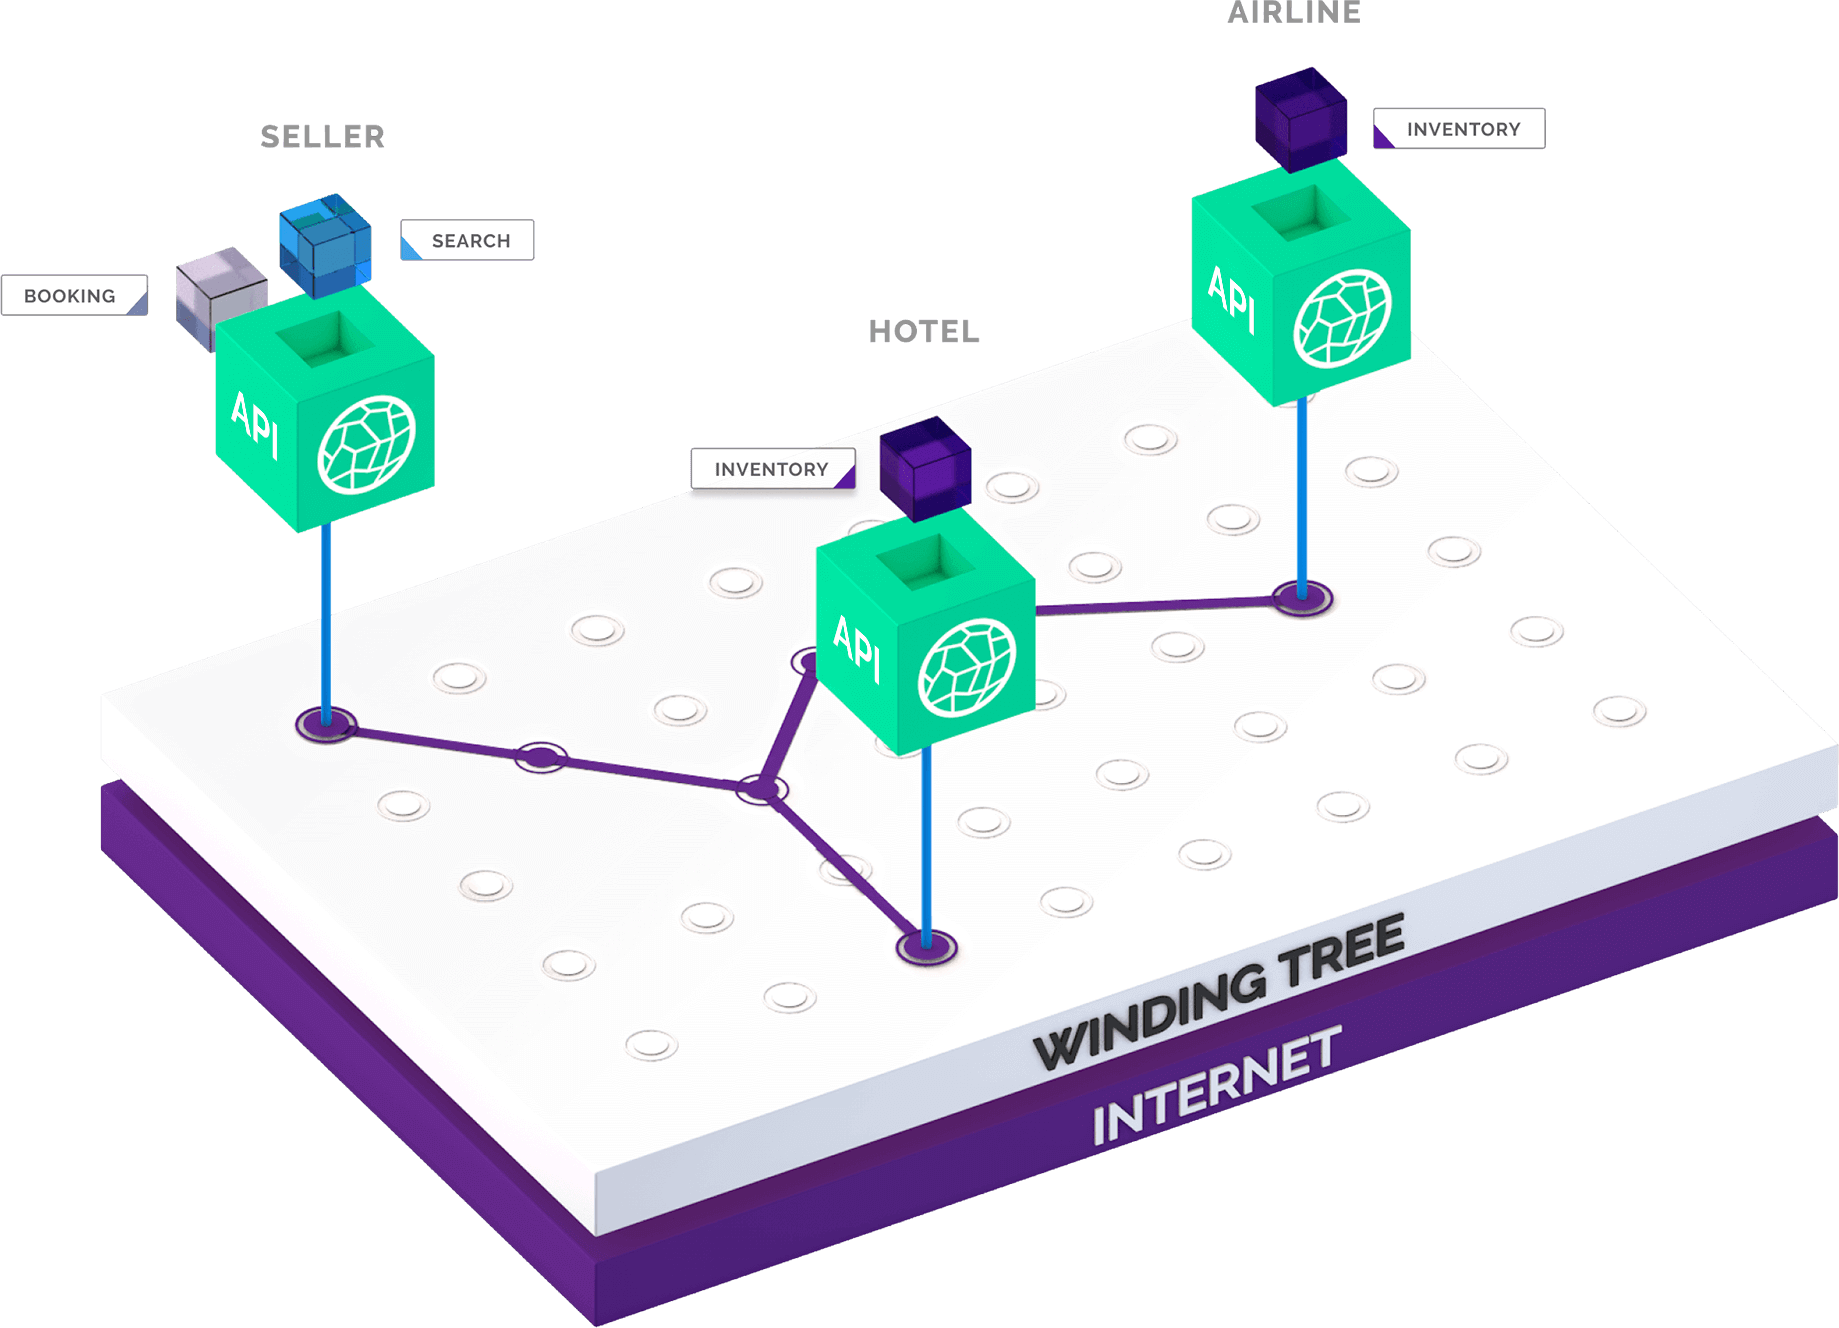
\includegraphics[width=\textwidth]{Bilder/WindingTreeOverview.png}
  \caption[Winding Tree Überblick]{Winding Tree Überblick \cite{WTWebsite2019}}
  \label{fig:windingTreeOverview}
\end{figure}

Winding Tree bietet lediglich die Plattform inklusive Schnittstellen zur Abwicklung der Geschäftsbeziehungen an, alle weiteren Anwendungen (z. B. Benutzeroberflächen) müssen von den Teilnehmern selbst implementiert werden. Dabei stehen als Hilfestellung allerdings auch Referenzimplementierungen in JavaScript unter der Apache-2.0-Lizenz auf Winding Trees GitHub Account bereit \cite{WTGitHub2019}.\\
Dass dies nicht nur eine Nischenlösung ist, wird beim Blick auf die Industriepartner bewusst: Neben Hotelketten wie Nordic Hotels sind vor allem große europäische Airlines auf der Plattform vertreten. Dazu gehören unter anderem auch AirFrance, KLM, SWISS, Eurowings und die Lufthansa \cite{WTWebsite2019}.

Eigens für die Plattform wurde der Líf Token generiert, welcher mehr Daten als ein typischer ERC20 Token verarbeiten kann und dabei die Kompatibilität beibehält \cite[][S. 9]{WT2019}. Dadurch können die für Reisen benötigten Daten kostengünstiger verarbeitet werden.\\ 
Zudem ergibt sich der Nebeneffekt der Plattformfinanzierung, was 2018 in Form eines Token Generation Events umgesetzt wurde. In mehreren Stadien konnten Ether in Líf umgewandelt werden. In der ersten Woche wurden 1000 Líf je Ether ausgeschüttet, in der zweiten Woche noch 900. Dabei wird die Anzahl der generierten Token vom Markt bestimmt. Stand heute (26. Juni 2019) ist ein Líf zum Preis von 0.0003 ETH respektive 0.91831 Eurocent erhältlich \cite{Coinmarketcap2019}. Um die laufenden Kosten für die Entwicklung der gemeinnützigen Firma Winding Tree tragen zu können, wurde zudem ein Marktvalidierungsmechanismus eingebaut. Dieser ist in Form eines autonomen Smart Contracts angelegt, welcher die Kapitalisierung, die die Marke von umgerechnet zehn Millionen US-Dollar zum Token Generation Event überschritten hat, verwaltet. Anhand einer festgelegten Preisfunktion werden Token angekauft und direkt vernichtet. Heute (Stand 26. Juni 2019) werden dort noch 4189 Ether, umgerechnet mehr als eine Million Euro, vorgehalten \cite{Lif2019}. Anhand [vgl.][S. 12 ff.]{WT2019}. \\
Somit gilt Líf als Wertinstrument für alle abzuwickelnden Tätigkeiten, die auf dem System stattfinden sollen. Am besten wird das am Beispiel aus Abbildung \ref{fig:windingTreeExample} deutlich.\\

\begin{figure}[h!]
  \centering
  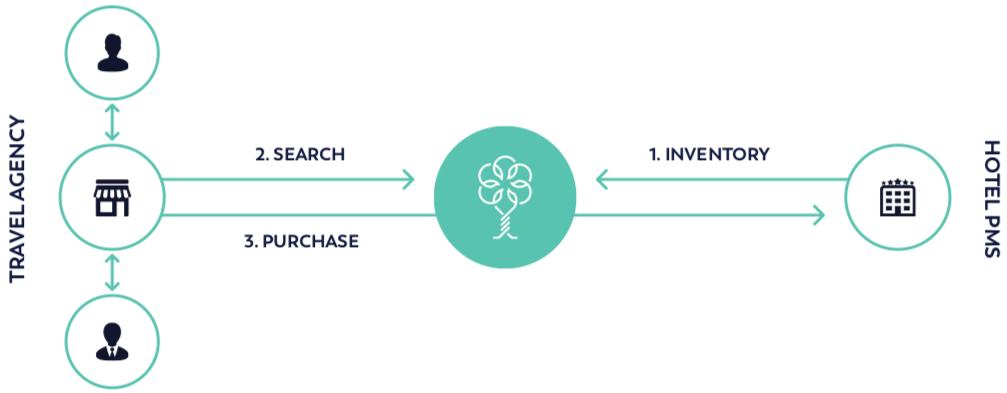
\includegraphics[width=\textwidth]{Bilder/WindingTreeExample.png}
  \caption[Beispiel eines Geschäftsfalls]{Beispiel eines Geschäftsfalls \cite[S. 10]{WT2019}}
  \label{fig:windingTreeExample}
\end{figure}

Um aus dem Property Management System des Hotels freie Zimmer an Winding Tree zu melden, muss eine zu diesem Zeitpunkt berechnete Menge an Líf gezahlt werden. Betrachet man die Smart Contracts und die API-Implementierungen aus dem oben bereits genannten GitHub Account, wird nicht sofort ersichtlich, wie diese Inventur getätigt wird. Die Contracts für die Airlines und Hotels sind relativ kurz gehalten und beschränken sich auf das Nötigste. Im Fall von Änderungen werden daher in der Regel nur Daten im Byteformat übertragen. Um die Zugriffe auf den Contract zu kapseln, und damit einfacher zu gestalten, dienen die angesprochenen APIs, welche in \emph{booking}, \emph{notification}, \emph{write} und \emph{read} unterteilt sind \cite[vgl.][]{WTAPIOverview2019}.\\
Um solche Änderungen einzupflegen müsste über den Contract zuerst ein Hotel im System angelegt werden. Dazu dient die Methode \texttt{registerHotel(...)}. Diese bindet das Hotel an einen \emph{manager}, der jedoch mittels \texttt{transferHotel(...)} das Hotel an eine andere Adresse übertragen kann. Über die \emph{write}-API werden schlussendlich die Daten des Hotels über die Methode \texttt{callHotel(...)} des Hotels überschrieben. \cite[vgl.][]{WTHotelContract2019, WTInventory2019}\\
Nun ist das Hotel für eine etwaige Reiseagentur über die Plattform auffindbar. Diese kann per \emph{read}-API potentielle Hotels abrufen. Momentan werden die Hotels in der Reihenfolge, wie sie in den Winding Tree Index geschrieben worden sind, ausgegegen. Somit lässt sich auch erst einmal nicht nach Hotels in der gewüschten geographischen Lage filtern, was durchaus problematisch werden könnte, wenn man kein Hotel als möglichen Kandidaten ausschließen will. Jedoch können unnötige Informationen über die Hotels auch mithilfe des Requests entfernt werden, d.h. z.B. lediglich die Blockchain-Adresse und die Koordinaten angezeigt werden, womit aber nicht das Problem des Abrufens letztendlich aller Hotels des Indexes gelöst wird. \cite[vgl.][]{WTQueryInventory2019}\\
Ist ein passendes Hotel gefunden, kann es gebucht werden. Dafür wird die \emph{booking}-API verwendet. Neben den Informationen über Gäste müssen auch Preisinformationen angefügt werden. Diese können aus den Daten der Plattform berechnet werden. Wieso die Daten nicht innerhalb eines Contracts beigefügt werden, ist unklar. \cite[vgl.][]{WTBooking2019}\\
Um auf Hotelseite die Buchung zu akzeptieren, muss eine sogenannte \texttt{bookingUri} hinterlegt sein. Um das einzutragen, sei an dieser Stelle auch wieder auf die \texttt{callHotel(...)}-Methode des dazugehörigen Smart Contracts verwiesen. Die URI zeigt auf ein hotelinternes System, welches eine REST API aufspannt, welche wiederum die Buchungsschnittstelle abbildet. An den Endpunkten der Schnittstelle kann dann eine Buchung hinterlegt, bzw. im Zweifelsfall storniert werden. \cite[vgl.][]{WTBookingAccept2019}

Als Abschluss dieses Kapitels sollen nochmals kurz einzelne Punkte aufgegriffen werden.\\
Positiv anzumerken ist das Verfügbarmachen aller Implementierungen. Von den Contracts bis hin zu den Schnittstellen-Implementierungen kann alles nachvollzogen werden. Bei Bedarf besteht die Möglichkeit, tiefer in das System einzusteigen. Ob jedoch die Öffnung des Quellcodes zu mehr Sicherheit beiträgt, ist umstritten. Die Möglichkeit, auf Schwachstellen aufmerksam machen zu können, ist dennoch hervorzuheben und bekräftigt die Ausrichtung Winding Trees zu offenen Softwaresystemen, wie der Ethereum Blockchain. Durch namhafte Kooperationen und eine im Voraus geplante Finanzierung, ist diese Smart Contract Anwendung durchaus als ernsthaft und positiv zu betrachten.\\ 
Dennoch wird aus den Reihen der Reisebranche auch Kritik laut.

%- Líf-Token -> Notwendigkeit, Grundlage, ganz kurz Token Event; Market Validation Mechanism interessanter [Seite 2 und 3 halb] \\ % https://windingtree.com/White_Paper_EN.pdf
%- Ablauf allgemein (Beispiel aus Whitepaper) + Contracts genauer (siehe GitHub) [Seite 3 halb und 4]\\#
%- Kritik am System [Seite 4] \\